\subsection{Mapping CML to UML and OCL}\label{subsec:mapping}

Part of the CML metamodel (presented in section \ref{subsec:metamodel}) may be considered a small subset of the UML  \cite{uml} metamodel.
Thus, the structural (static) elements of CML models can be transformed into UML class diagrams. The example CML model in the listing of figure \ref{fig:store} is mapped to the UML model in figure \ref{fig:uml}.

\begin{figure}
\centering
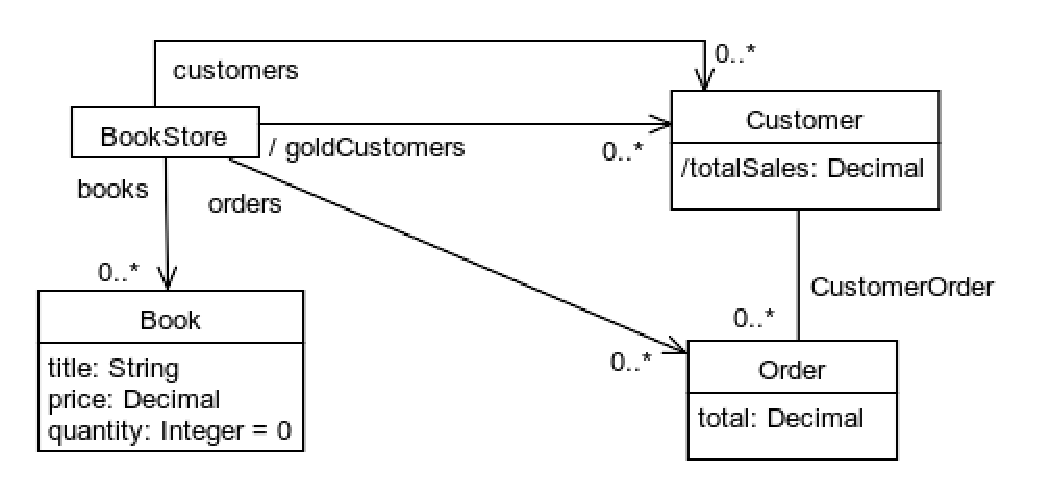
\includegraphics[width=0.8\textwidth]{language/diagram-uml}
\caption{The class diagram representing in UML  \cite{uml} the same CML model listed in figure \ref{fig:store}.}
\label{fig:uml}
\end{figure}

In the UML class diagram of figure \ref{fig:uml}:
\begin{itemize}
\item the CML concepts (\emph{BookStore}, \emph{Book}, \emph{Customer} and \emph{Order}) are mapped to corresponding UML classes;
\item the CML properties that represent attributes
(such as \emph{title}, \emph{quantity} and \emph{price} of \emph{Book})
are mapped to corresponding UML attributes under each class;
\item the CML properties that represent unidirectional associations
(\emph{books}, \emph{customers}, and \emph{goldCustomers} of \emph{BookStore})
are mapped to UML associations with corresponding roles
(showing the navigability direction, and matching the property names);
\item the CML bidirectional association \emph{CustomerOrder}
(comprised by two CML properties: \emph{Customer.orders} and \emph{Order.customer})
is mapped to a UML association with bidirectional navigability (no direction arrow).
\end{itemize}

As demonstrated by this example,
CML strives to enable modeling at the same conceptual level as allowed by UML.
When compared to the UML metamodel,
the CML metamodel supports only a core set of its elements (as shown in subsection \ref{subsec:metamodel}).
This minimally viable core has been intentionally designed to validate CML's objectives.

Besides the structural elements of a conceptual model (as seen above),
CML also permits the use of expressions to set initial values to attributes,
and to define derived properties for both attributes and associations.
These expressions are partially based on the OCL \cite{ocl} syntax,
but they follow closely the OCL semantics,
as described in section \ref{subsec:expr}.

For example, the following CML expression (extracted from figure \ref{fig:store}) is a path-based navigation expression borrowed from OCL:

\begin{verbatim}
/orderedBooks = orders.items.book;
\end{verbatim}

Using association properties, the expression above navigates from one instance of \emph{BookStore}, passing through all linked \emph{orders}, and then through all \emph{items} of all \emph{orders}, in order to return all books that have been ordered. (The semantics of path expressions will be given in section \ref{subsec:expr}.)

As another example,
the following CML expression (also extracted from figure \ref{fig:store}) does not follow the OCL syntax:

\begin{verbatim}
/goldCustomers = customers | select totalSales > 1000;
\end{verbatim}

However, the expression above closely matches the semantics of the following OCL expression:

\begin{verbatim}
derive: customers->select(totalSales > 1000)
\end{verbatim}

Both the CML expression and the OCL excerpt above evaluate to a set of \emph{Customer} instances
that have bought more than 1000 in the \emph{BookStore}. 

As with path expressions, the semantics of all expressions will be shown in section \ref{subsec:expr}.
 